\section{Annex}
\subsection{Screen shots}

\begin{figure}[h]
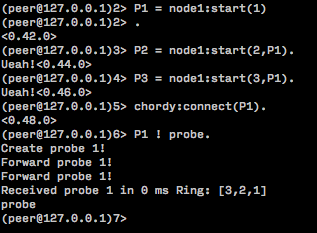
\includegraphics[scale=1.0]{node1Works.png}
\centering
\caption{Node1 - Working}
\end{figure}

\begin{figure}[h]
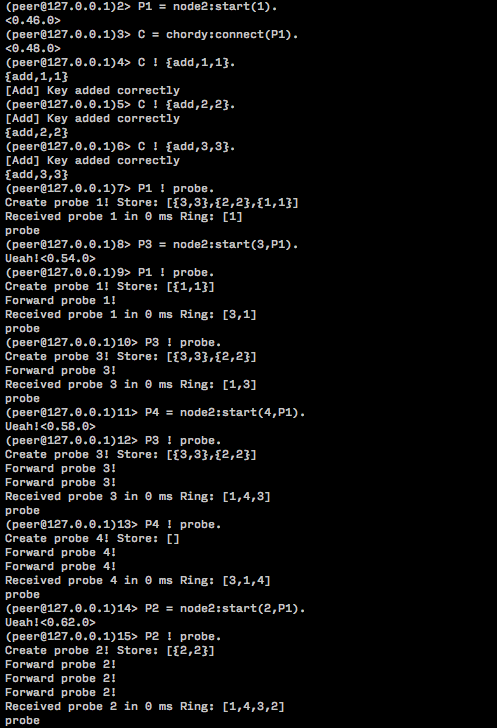
\includegraphics[scale=0.8]{node2Full.png}
\centering
\caption{Node2 - Working correctly, full example}
\end{figure}

\begin{figure}[h]
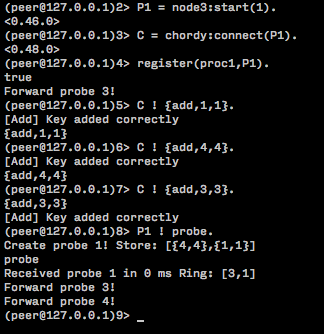
\includegraphics[scale=1.0]{node3works1.png}
\centering
\caption{Node3 - Peer1 (distributed)}
\end{figure}

\begin{figure}[h]
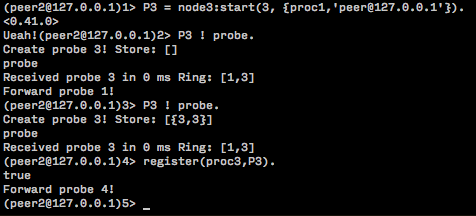
\includegraphics[scale=1.0]{node3works2.png}
\centering
\caption{Node3 - Peer2 (distributed)}
\end{figure}

\begin{figure}[h]
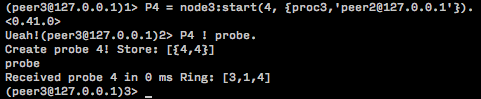
\includegraphics[scale=1.0]{node3works3.png}
\centering
\caption{Node3 - Peer3 (distributed)}
\end{figure}

\begin{figure}[h]
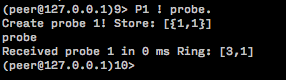
\includegraphics[scale=1.0]{node3works1_nodeDown.png}
\centering
\caption{Node3 - Peer1, Peer3 down (distributed), ring OK}
\end{figure}

\begin{figure}[h]
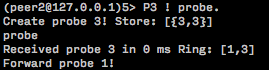
\includegraphics[scale=1.0]{node3works2_nodeDown.png}
\centering
\caption{Node3 - Peer2, Peer3 down (distributed), ring OK}
\end{figure}

\begin{figure}[h]
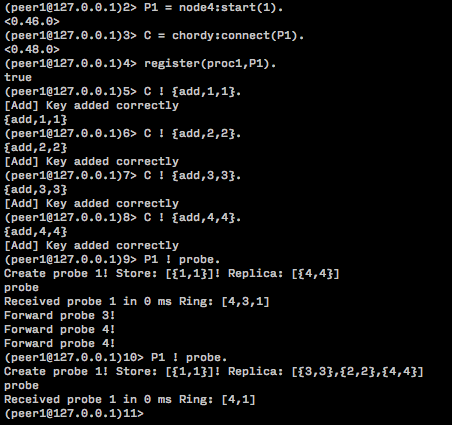
\includegraphics[scale=1.0]{node4works1+peer2down.png}
\centering
\caption{Node4 - Peer1 (distributed), ring OK when Peer2 down}
\end{figure}

\begin{figure}[h]
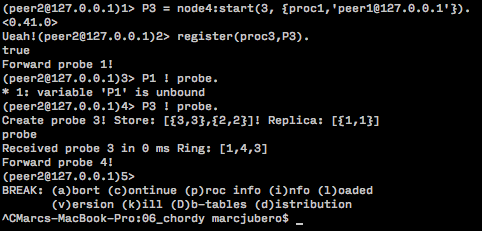
\includegraphics[scale=1.0]{node4works2+peer2down.png}
\centering
\caption{Node4 - Peer2 (distributed), ring OK when Peer2 down}
\end{figure}

\begin{figure}[h]
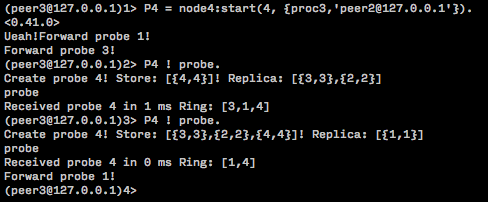
\includegraphics[scale=1.0]{node4works3+peer2down.png}
\centering
\caption{Node4 - Peer3 (distributed), ring OK when Peer2 down}
\end{figure}


\begin{figure}[h]
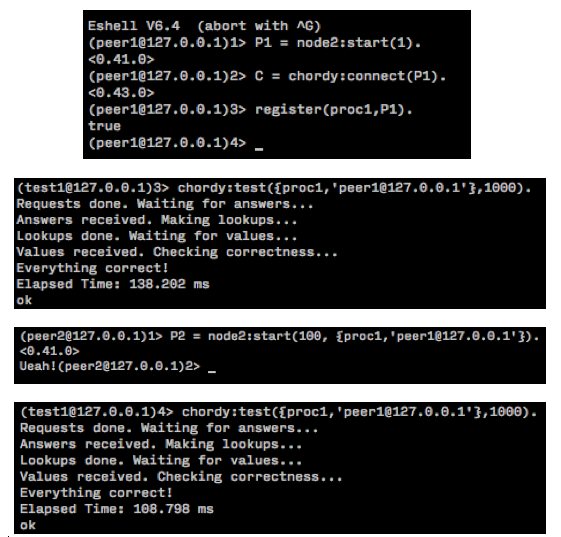
\includegraphics[scale=0.8]{321_concat.png}
\centering
\caption{Test performance: Single node 138.202ms ; Two nodes 108.798ms}
\end{figure}

\begin{figure}[h]
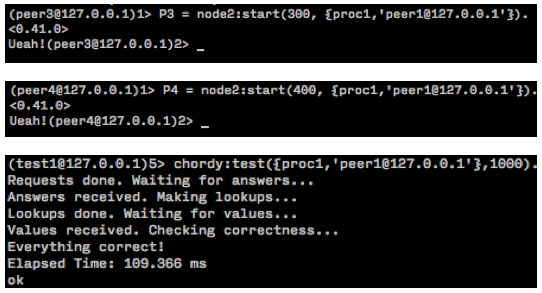
\includegraphics[scale=0.8]{322_concat.png}
\centering
\caption{Test performance: add 2 more nodes}
\end{figure}

\begin{figure}[h]
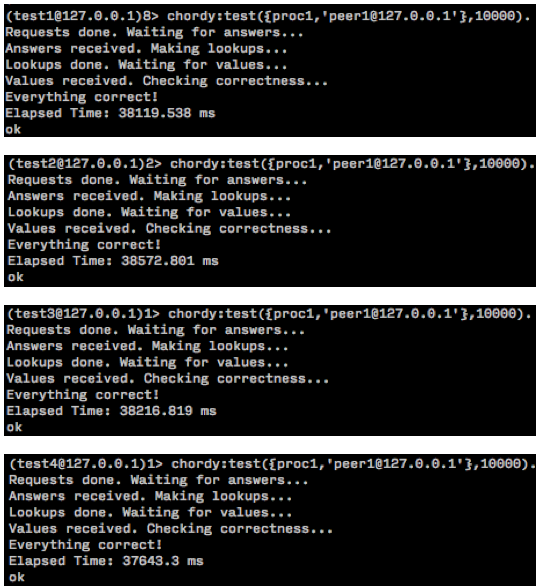
\includegraphics[scale=0.8]{tests_allToOne.png}
\centering
\caption{Test performance: 4 nodes, 4 test clients launching tests over peer1}
\end{figure}

\begin{figure}[h]
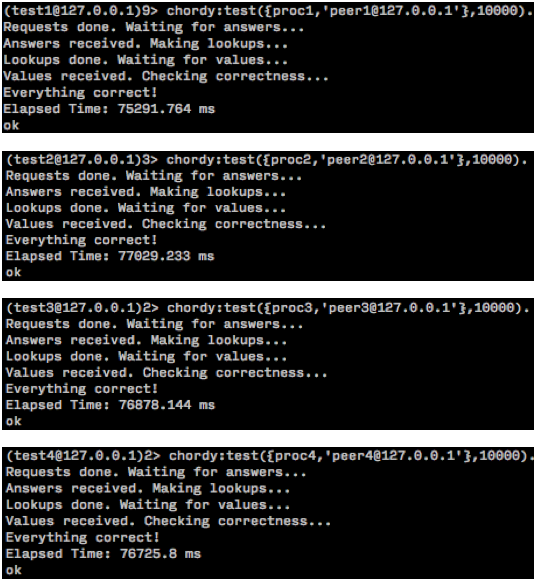
\includegraphics[scale=0.8]{tests_distrib.png}
\centering
\caption{Test performance:4 nodes, 4 test clients launching tests. 1 test client to 1 node}
\end{figure}


































\clearpage

\subsection{Source code}
\subsubsection{node1}
\inputminted[
    fontsize=\medium,
    linenos]{erlang}{resources/src/node1.erl}

\clearpage
\subsubsection{node2}
\inputminted[
    fontsize=\medium,
    linenos]{erlang}{resources/src/node2.erl}

\clearpage
\subsubsection{node3}
\inputminted[
    fontsize=\medium,
    linenos]{erlang}{resources/src/node3.erl}

\clearpage
\subsubsection{node4}
\inputminted[
    fontsize=\medium,
    linenos]{erlang}{resources/src/node4.erl}
